\documentclass{article}
\usepackage[utf8]{inputenc}
\usepackage[T1]{fontenc}
\usepackage{amsmath}
\usepackage{url}
\usepackage{listings}
\usepackage{xcolor}
\usepackage{graphicx}
\usepackage{parskip}
\usepackage[toc,page]{appendix}

\definecolor{codegreen}{rgb}{0,0.6,0}
\definecolor{codegray}{rgb}{0.5,0.5,0.5}
\definecolor{codepurple}{rgb}{0.58,0,0.82}
\definecolor{backcolour}{rgb}{0.95,0.95,0.92}

\lstdefinestyle{mystyle}{
    backgroundcolor=\color{backcolour},   
    commentstyle=\color{codegreen},
    keywordstyle=\color{magenta},
    numberstyle=\tiny\color{codegray},
    stringstyle=\color{codepurple},
    basicstyle=\ttfamily\footnotesize,
    breakatwhitespace=false,         
    breaklines=true,                 
    captionpos=b,                    
    keepspaces=true,                 
    numbers=left,                    
    numbersep=5pt,                  
    showspaces=false,                
    showstringspaces=false,
    showtabs=false,                  
    tabsize=2
}
\lstset{style=mystyle}

\author{Wenhao LUO}
\title{Procédure de remise}
\begin{document}
\maketitle
\date{}

\cleardoublepage
\tableofcontents

\clearpage

\section{Introduction}
\par En suivant le cours \textbf{8INF878-Intelligence Artificielle} de l'Université de Québec à Chicoutimi, on a réalisé ce projet "compétition d'agent intelligents pour le jeu d'échecs" par l'implémentation d'une intelligence artificielle comme un engine jouable sur la plateforme ARENA.

\par Ce document sert à introduire le fonctionnement de ce programme, à expliquer comment on a réalisé cette implémentation et à discuter les difficultés rencontrés pendant la réalisation de ce projet.

\section{Fonctionnement du programme}

\subsection{Informations générales}
\par Le programme réalisé, nommé \texttt{OCAP} est un engine qui est capable de jouer le jeu d'échecs avec l'aide du logiciel ARENA. Il est capable de comprendre une partie des commandes définies avec le protocole UCI, qui le permet de reconstituer, d'analyser et de jouer un jeu d'échecs avec les données transmis par \texttt{stdin} et \texttt{stdout}.

\subsection{Commandes acceptées} \label{commandes}
\par Voici la liste de toutes les commandes qui peuvent être insérées et comprises par ce logiciel :
\begin{itemize}
    \item \texttt{uci} : en acceptant cette commande, le programme retourne son identifiant et son auteur ;
    \item \texttt{isready} : en acceptant cette commande, le programme retourne le message "isready" qui permet de confirmer qu'il est prêt au calcul ;
    \item \texttt{go} : en acceptant cette commande, le programme commence à effectuer les calculs ; il devra retourner un résultat plus tard avec un délai prédéfini ;
    \item \texttt{stop} : en acceptant cette commande, le programme arrête son calcul et il retourne un résultat le plus vite possible ;
    \item \texttt{quit} : en acceptant cette commande, le programme arrête son fonctionnement et termine l'exécution de tous les threads ;
    \item \texttt{position startpos [moves] <move1>, <move2>, ...} : en acceptant cette commande, le programme reconstitue un damier au sein du programme, qui permet de réaliser les calculs plus tard.
\end{itemize}

\subsection{Interaction avec ce programme}
\par Avec l'interface ARENA, une personne peut jouer un jeu d'échecs avec ce programme en le chargeant comme un des engines de l'ARENA. C'est également possible de jouer le jeu directement en lançant ce programme dans une ligne de commande par insérer les commandes listées dans la section \ref{commandes}.


\section{Implémentation}

\subsection{Langage et paradigme utilisé}
\par Le programme est écrit en Java, et naturellement avec le paradigme OOP. Certaines parties sont écrites avec multithreading.

\subsection{Topologie du programme}
\par Le programme peut être séparé en trois parties différentes :
\begin{itemize}
    \item un damier et des pièces de l'échecs construct au sein du système, qui permet de reconstruire un scénario du jeu et l'évaluer ;
    \item un programme qui permet d'analyser le meilleur choix dans une situation donnée, et de prendre des décisions ;
    \item un parseur minimise qui permet de comprendre les commandées entrées et de communiquer avec les autres composantes du programme.
\end{itemize}

\par Prochainement on va parler des trois parties à l'ordre.

\subsection{Damier et pièces}
\par La première partie du programme réalise un damier de l'échecs \texttt{Board} avec des pièces qui peuvent être mises sur un damier. Un damier contient une liste de pièces et leur coordonnées, qui est un "état" du jeu. J'ai également implémenté les fonctions qui permettent de réaliser les fonctionnements basiques, comme une fonction qui retrouve une liste des actions légales, et une autre fonction qui permet de réaliser une transition entre deux états. Les exemples peuvent être retrouvés dans le listing \ref{lst:board}.

\par Des pièces du jeu sont programmés avec un héritage de classe : toutes les pièces sont considérées comme un membre de la classe \texttt{Piece}, ensuite chaque pièce réalise ses propres méthodes. Le code de la classe \texttt{Piece} est disponible comme le listing \ref{lst:piece}.

\par Le problème de gestion de mémoire a été pris en compte pendant le développement. Notons que dans la classe \texttt{Board} les pièces ne sauvegardent pas leur position sur le damier ; en fait il ne sauvegarde non plus l'objet \texttt{Board}. J'ai choisi cette implémentation afin d'éviter de recopier les objets \texttt{Piece} entre la transition des deux damiers.

\par Si un nouveau état du jeu doit être créé en déplaçant une pièce sur un damier, alors seulement la position des pièces sera modifié ; les différents damiers partagent les mêmes pièces : chaque fois on trace la position des pièces par un nouveau dictionnaire et tous les dictionnaires pointent les mêmes objets. Une illustration est donnée comme le figure \ref{fig:copies}.

\begin{figure}[htb]
    \centering
    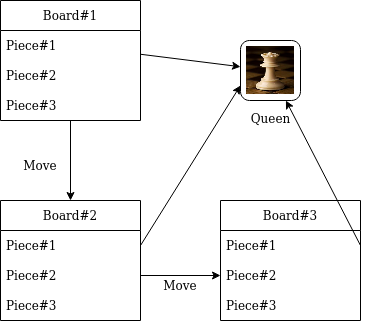
\includegraphics[width = 0.7\linewidth]{illustation.png}
    \caption{Illustration sur la création des nouveaux états.}
    \label{fig:copies}
\end{figure}

\par La classe \texttt{Board} génère toutes les possibles actions à partir des positions des pièces. Les actions sont nommées comme \texttt{Move}. Un damier peut généré un nouveau damier selon une instance de \texttt{Move} donnée. On est donc capable de décrire les différents états et leur transition.

\subsection{Analyseur}
\subsubsection{Algorithme utilisé}
\par On utilise une recherche en appliquant un algorithme élagage alpha-bêta\cite{enwiki:Alphabeta}. Le principe de cet algorithme est d'explorer les différents nœuds par profondeur, en applicant une optimisation supplémentaire en mémorisant deux valeurs $\alpha$ et $\beta$. Ces valeurs représentent les meilleurs/pires cas possibles. Si le résultat retrouvé par un nœud dépasse ces valeurs, alors théoriquement ces nœuds seront jamais visités, supposant que les joueurs ne choisissent que les meilleurs choix. Ainsi on évite de faire les visites non nécessaires.

\subsubsection{Fonction d'évaluation}
\par Une fonction d'évaluation est nécessaire pour déterminer si un état est "bon" ou "mauvais". C'est le facteur plus important sur la qualité de notre programme. Heureusement il y a déjà les recherches sur ce domaine, et on a un système d'évaluation classique qui affecte une note sur chaque pièce sur un damier. C'est le \textit{chess piece relative value}\cite{enwiki:value}. Selon ce système, on affecte une note de la manière présentée dans le tableau \ref{tab:score}. D'ailleurs, puisque la perte des "Roi" cause la perte du jeu, on lui affecte une note de $\infty$. Les notes sont présentés en nombre flottant ; la valeur d'infinie est donc bien définie dans le contexte.

\par C'était la première implémentation que on a réalisée. Pourtant on trouve que cette implémentation ne permet pas de distinguer la qualité des différents choix au début du jeu : théoriquement l'échange des pièces n'est pas souvent spécialement au début du jeu, et cette évaluation ne peut pas trouver le meilleur choix dans ce cas. Pour résoudre ce problème, on a introduit une nouvelle fonction heuristique. Soit $d_1$ la distance entre une case et l'arête \texttt{a1-h1} et $d_2$ la distance entre une case et l'arête \texttt{a8-h8}, $h_c$ un constant. La fonction $h$ est définie par l'équation \ref{equ:h}.

\begin{equation}\label{equ:h}
    h = \left\lbrace
    \begin{array}{lr}
        h_c \left\lvert d_1 - 5 \right\rvert & si \ p \in White \\
        h_c \left\lvert d_2 - 2 \right\rvert & si \ p \in Black
    \end{array}
    \right.
\end{equation} 

Autrement dit, la plus avancée une pièce est, la meilleure note qu'elle est affectée. Ceci permet de progresser le jeu et d'éviter les boucles. Après les tests, on a décidé de mettre $h_c = 0.1$.

\begin{table}
    \centering
    \begin{tabular}[htb]{|c|c|}
        \hline
        Type & Valeur \\
        \hline
        Pion & 1 \\
        \hline
        Cavalier & 3 \\
        \hline
        Fou & 3 \\
        \hline
        Tour & 5 \\
        \hline
        Dame & 9 \\
        \hline
    \end{tabular}
    \caption{Les notes en fonction des pièces.}
    \label{tab:score}
\end{table}

\subsubsection{Application multithread}
\par L'algorithme alpha-bêta est implémenté sous la forme d'une fonction récursive. La fonction de exploration fait son calcul de façon continue. On a besoin de lancer cette fonction par un thread séparé, afin d'arrêter le calcul quand l'interface émet le signal de terminaison. C'est-à-dire le commande \texttt{stop} discutée dans la section \ref{commandes}.

\par On réalise la synchronisation par une variable partagée entre plusieurs threads. Une variable booléenne \texttt{isFinish} est déclarée au moment de l'instanciation. Le thread principal peut modifier sa valeur quand la recherche est terminée ; le thread qui réalise la recherche vérifie la valeur de cette variable quand il fait l'appel récursive. Ce mécanisme permet donc de terminer l'exploration instantanément.

\par Si on interrompe le thread au milieu d'une exploration, alors l'exploration n'est pas complète. Le résultat n'est pas fidèle. Pour résoudre ce problème, l'exploration est faite de façon progressive. On commence par un profondeur de $k$, une fois le calcul est fini on sauvegarde le résultat et on continue par un profondeur de $k+1, k+2, \cdots$. Le code est présenté dans le listing \ref{lst:recherche}.

\subsection{Communication}

\section{Difficultés rencontrés}

\section{Conclusion}

\clearpage
\bibliographystyle{plain}
\bibliography{refs}

\clearpage
\begin{appendices}
\section{Code implémenté}

\begin{lstlisting}[language=java, caption={Une partie des fonctions réalisées dans la classe \texttt{Board}.}, label={lst:board}]
public class Board implements Cloneable {

    private final double heuristicConst = 0.1;

    private HashMap<PieceType, ArrayList<Piece>> availablePieces = new HashMap<>();
    private TreeMap<Coord, Piece> board = new TreeMap<>();

    private boolean isBlackMove = false;
    
    public Coord enpassant = null; // null means no "enpassant"
    // otherwise is the last coord of the "enpassant"
    // these variables are used to track the "castling"
    // zero for black, one for white
    private boolean[] isKingMoved = {false, false};
    private boolean[] isLeftRockMoved = {false, false};
    private boolean[] isRightRockMoved = {false, false};

    public boolean isBlackMove() {...}
    public TreeMap<Coord, Piece> getWhitePieces() {...}
    ...
}
\end{lstlisting}

\begin{lstlisting}[language=java, caption={La classe abstracte \texttt{Piece}.}, label={lst:piece}]
package Board;

import java.util.TreeSet;

import mUtil.Coord;

public abstract class Piece {
    protected boolean isBlackVal;
    abstract public TreeSet<Coord> getLegalMoves(Board currentBoard, Coord currentCoord);

    abstract public String getShortName();
        
    public Piece(boolean isBlack) {
        this.isBlackVal = isBlack;
    }
    
    public boolean isBlack() {
        return isBlackVal;
    }

}
\end{lstlisting}

\begin{lstlisting}[language=java, caption={La recherche récursive, réalisée par un thread séparant.}, label={lst:recherche}]

@Override
public void run() {
    int depth = 1;
    while (!isFinish && depth <= depthLimit) {
        explore(depth);
        depth += 1;
        System.out.format("info depth %d finish\n", depth);
        this.oldRoot = this.root;
        this.root = new Node(board);
    }
}
    
\end{lstlisting}

\end{appendices}

\end{document}
